

\chapter{Casi d'uso}                %crea il capitolo
%%%%%%%%%%%%%%%%%%%%%%%%%%%%%%%%%%%%%%%%%imposta l'intestazione di pagina
\lhead[\fancyplain{}{\bfseries\thepage}]{\fancyplain{}{\bfseries\rightmark}}
Di seguito alcuni esempi di utilizzo della libreria.
Le dimostrazioni seguenti sono state effettuate su una macchina con architettura amd64 e con installato il sistema operativo debian in versione sid (quindi unstable) ma sono state testate e riprodotte anche su altre configurazioni e distribuzioni GNU/Linux.
\section{Environment}
Come precedentemente accennato possiamo integrare la nostra libreria in vuos attraverso il modulo unrealvsnlib o creandone uno alternativo che dipenda da questa VsnLib.\\
\begin{description}
\item[Creazione moduli:] La creazione di un modulo \`e molto semplice e basta serguire le linee guida di quelli preesisteni, inoltre grazie ad una routine in cmake non \`e necessario aggiungere alcuna riga manualmente al makefile e sar\`a, appunto, cmake ad occuparsi della compilazione.
\item[Start Vuos:] Vuos si avvia attaverso il comando umvu ed \`e in grado di interpretare comandi successivi come argomenti, come mostrato nell'esempio infatti umvu \`e affiancato dal comando xterm e pertanto verr\`a lanciata una nuova istanza di terminale con ambiente vuos. Nel caso specifico \`e stato utilizzato il programma konsole, Il risultato non cambia; in alternativa anche bash o zsh andrebbero bene ma si perderebbero le informazioni mostrate da vuos nel primo terminale.
\item[Include dei Moduli vuos] I moduli in vuos vengono inclusi attraverso la direttiva
\begin{verbatim}
vu_insmode <nome_modulo>
\end{verbatim}
Un esempio di avvio e inclusione del modulo \`e quello della figura seguente.
\begin{figure}[h]                       %crea l'ambiente figura; [h] sta
                                        %   per here, cio� la figura va qui
\begin{center}                          %centra nel mezzo della pagina
                                        %   la figura
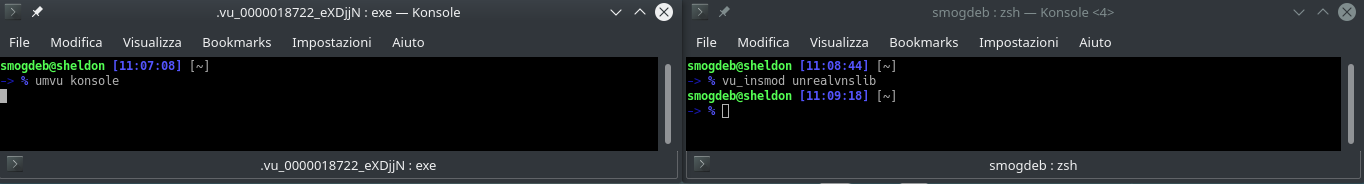
\includegraphics[width=16cm]{start_vuos}%inserisce una figura larga 5cm
                                        %se si vuole usare va scommentata
%
%%%%%%%%%%%%%%%%%%%%%%%%%%%%%%%%%%%%%%%%%inserisce la legenda ed etichetta
                                        %   la figura con \label{fig:prima}
\caption[start/include\_mod vuos]{start and include vuos}\label{fig:map}
\end{center}
\end{figure}
\end{description}
\section{Esempi}                 %crea la sezione

%%%%%%%%%%%%%%%%%%%%%%%%%%%%%%%%%%%%%%%%%non numera l'ultima pagina sinistra
\clearpage{\pagestyle{empty}\cleardoublepage}
